\documentclass[10pt]{article}
\usepackage[letterpaper, margin=1in]{geometry}
\usepackage[pdftex]{graphicx}
\usepackage[utf8]{inputenc}
\usepackage{tikz, wrapfig, amssymb, array, mathtools, circuitikz, physics, parskip, hyperref}
\usepackage{enumerate}
\usepackage{tkz-euclide}
\usepackage{titlesec}
\usepackage{lipsum}
\usepackage[english]{babel}
\usepackage{amsmath, amsthm}
\usepackage{fancyhdr}
\usepackage{xcoffins}
\usepackage{tcolorbox}
\usepackage{../local}


\newcommand{\classcode}{Physics 5C}
\newcommand{\classname}{Introductory Thermodynamics and Quantum Mechanics}
\renewcommand{\maketitle}{%
\hrule height4pt
\large{Eric Du \hfill \classcode}
\newline
\large{HW 07} \large{\hfill \classname \hfill} \large{\today}
\hrule height4pt \vskip .7em
\normalsize
}
\linespread{1.1}
\begin{document}
    \maketitle

    \section*{Collaborators}

    I worked with \textbf{Andrew Binder, Nathan Song, Teja Nivarthi, Nikhil Maserang,} and \textbf{Christine Zhang} to complete this assignment.
    \section*{Problem 1}

    A particle of mass $m$ has $N$ quantized energy levels in a one-dimensional square well of depth $V_0$ and width $L$. $N$ is more than 10.

    \begin{enumerate}[(a)]
        \item Approximately how many bound states does the particle have in a well of the same depth but width $2L$?

        \begin{solution}
            There are twice as many bound states ($2N$) when we double the width, because we can now fit twice as many nodes into the same well, giving us twice the number of energy levels. This is due to the node theorem in Quantum Mechanics.
        \end{solution}
        \item Approximately how many states does the particle have in a well of width $L$ but depth $2V_0$?
        
        \begin{solution}
            Because the energy scales with $n^2$ instead of $n$, then doubling the depth of the well does not double the number of energy levels but raises it by $\sqrt{2}N$. 
        \end{solution}
        \item Approximately how many states does the particle have in a well of depth $2V_0$ and width $2L$?
        
        \begin{solution}
            Using the logic of the previous two problems, then we know that doubling the depth doubles the number of bound states, then increasing the width increases this by a further factor of $\sqrt 2$. Therefore, the final number of bound states is $2\sqrt{2}N$.
        \end{solution}
        \item How many bound states does the particle have in a well of depth $V_0/4$ and width $2L$? In a well of depth $4V_0$ and width $L/2$?
        
        \begin{solution}
            Again, using the logic of parts (a) and (b), then decreasing the depth of the well exactly cancels out increasing the width exactly, so therefore the number of bound states doesn't change in both cases.
        \end{solution}
    \end{enumerate}

    \pagebreak

    \section*{Problem 2}

    A particle is bound in a one-dimensional well with one rigid wall whose potential is shown in the figure.


    \begin{center}
        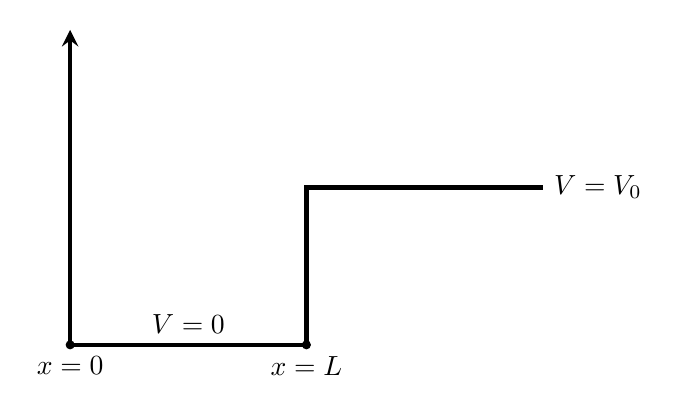
\begin{tikzpicture}
            \draw[ultra thick, -stealth] (0,0) node[anchor=north] {$x = 0$} -- (0,4);
            \draw[ultra thick] (0,0) -- (3,0) node[midway, above] {$V = 0$} node[anchor=north] {$x = L$} -- (3,2) -- (6,2) node[anchor=west] {$V = V_0$};
            \filldraw[black] (0,0) circle (0.05cm);
            \filldraw[black] (3,0) circle (0.05cm);
        \end{tikzpicture} 
    \end{center}x

    \begin{enumerate}[(a)]
        \item For $E < V_0$, write down and solve the \schrodinger equation for the region inside the well and the region outside the well. 
        
        \begin{solution}
            Inside the well, the \schrodinger equation is solved using $V(x) = 0$, so therefore we have scattering states: 

            \[ \psi(x) = A \cos(kx) + B \sin (kx), \phantom{aa} k = \left(\frac{2mE}{\hbar^2}\right)^{1/2}\]

            Outside the well on the left, because the potential is infinite, then $\psi_L(x) = 0$ is the only solution. On the right of the well, we get an evanescnent wave, so therefore 

            \[ \psi_R(x) = Ce^{-\alpha x}, \phantom{aa} \alpha = \left(\frac{2m(V_0 - E)}{\hbar^2}\right)^{1/2}\]
        \end{solution}
        \item Apply the boundary conditions at $x=0$ and $x = L$ to obtain an equation that defines the allowed values of the energy $E$. 
        
        \begin{solution}
            We will take the odd solutions, for simplicity. Therefore, we only have $\psi(x) = B\sin (kx)$ inside the well. This also matches the boundary condition at $x = 0$ automatically. 

            At $x = L$, we require continuity in $\psi$ and $\psi'$: 

            \begin{align*}
                \psi: B\sin(kL) &= Ce^{-\alpha L}\\
                \psi': Bk \cos (kL) &= -\alpha Ce^{-\alpha L}
            \end{align*}
            
            Dividing the two equations, we get: 

            \[ \frac{1}{k} \tan(kL) = \frac{1}{\alpha}\]

            which is an equation for the energy.
        \end{solution}
        \item Show that for $V_0$ very large, the permitted energies approach those for the infinite deep square well of width $L$.
        
        \begin{solution}
            For large $V_0$, then we have that $\alpha \to \infty$. Therefore, our equation becomes: 

            \[ \tan(kL) = 0\] 

            And therefore: 

            \begin{align*}
                kL &= n\pi\\
                \left(\frac{2mE}{\hbar^2}\right)^{1/2} &= \frac{n\pi}{L}\\
                \frac{2mE_n}{\hbar^2} &= \frac{n^2\pi^2}{L^2}\\
                \therefore E_n &= \frac{\hbar^2 n^2 \pi^2}{2mL^2}
            \end{align*}

            which is exactly the energy levels we get from an infinite square well.
        \end{solution}
        \item Introduce dimensionless quantities $\theta$ and $\theta_0$ according to Eqs. 4-5 and 4-6 of the text. By compareing the result with Eq. 4-8, show that the permitted energies of the "half-infinite" well of width $L$ are exactly the energies for the odd solutions of the finite well of the same depth $V_0$ but twice the width, $2L$. Explain how this arises out of the boundary condition at $x = 0$ for the half-infinite case.
        
        \begin{solution}
            We introduce $\theta = kL/2$ and $\theta_0 = \sqrt{2mV_0}{\hbar} \cdot L/2$. Now we take the reciprocal of our energy equation: 

            \[ \cot (2\theta) = -\frac{\alpha}{k}\]

            The ratio $\alpha/k$ is known, and so our equation simplifies to: 

            \begin{align*}
                \cot (2\theta) &= -\sqrt{\frac{V_0}{E} - 1}\\
                \cot (2\theta) &= -\sqrt{\left(\frac{\theta_0}{\theta}\right)^2 - 1}
            \end{align*}

            Equation 4-8 in the textbook reads 

            \[  \cot (\theta) = -\sqrt{\left(\frac{\theta_0}{\theta}\right)^2 - 1}\] 

            so notice that the only difference in these equations is in the fact that we have $\cot(\theta)$ and $\cot(2\theta)$. Therefore, our equation will only admit half as many solutions, becuase $\theta$ increases twice as fast. 

            Qualitatively, because our half-infinite square well cuts off at the left edge, we have no information about the wavefunction at $x < 0$. We can then ``stitch'' this solution together with a square well where the potential is infinity at $x > 0$ (which has no information). What this means is that we can imagine a finite square well as effectively a combination of these two potentials: 

            \begin{center}
                \begin{tikzpicture}
                    \draw[ultra thick, -stealth, dashed] (0,0) node[anchor=north] {$x = 0$} -- (0,4);
                    \draw[ultra thick] (-6,2) -- (-3,2) -- (-3,0) node[anchor=north] {$x = -L$} -- (0,0) -- (3,0) node[midway, above] {$V = 0$} node[anchor=north] {$x = L$} -- (3,2) -- (6,2) node[anchor=west] {$V = V_0$};
                    \filldraw[black] (0,0) circle (0.05cm);
                    \filldraw[black] (3,0) circle (0.05cm);
                    \filldraw[black] (-3,0) circle (0.05cm);
                \end{tikzpicture}
            \end{center}

            Then, we only get the odd solutions from this computation when compared to the full square well since we must enforce that $\psi(0) = 0$, so only odd solutions (when compared to the full finite square well) would fit in this framework. Then, we can then enforce continuity in $\psi$ and $\psi'$ to get a complete bound state for the finite square well. Therefore, we have shown that only the odd solutions exist in the half-infinite square well, as desired.


        \end{solution}
        \item For the case $\theta_0 = \pi$, or $V_0 = \hbar^2/(2mL^2)$, graphically solve the equation for the lowest permitted energy. Show that this is about three-quarters of the energy $\hbar^2/(8umL^2)$ that one would have for the infinitely deep well of width $L$. 
        
        \begin{solution}
            At $\theta_0 = \pi$, then we can numerically solve that the lowest value for $\theta = 1.3488$. Solving for the energy, we get: 

            \begin{align*}
                \frac{\sqrt{2mE}}{\hbar} \frac{L}{2} &= 1.34\\
                E_1 &= \frac{2(1.34)^2 \hbar^2}{mL^2}
            \end{align*}

            Using 3/4 of the energy given in the problem statement, then we get: 

            \[ E = \frac{3}{4} \frac{\pi^2\hbar^2}{2mL^2}\] 

            We note that $2(1.34)^2 \approx 3.59$ and $3\pi^2/8 \approx 3.70$, so they are relatively similar coefficients, and so they are more or less the same. 
        \end{solution}
        \item How many bound states are there altogether for the case $\theta_0 = \pi$?
        
        \begin{solution}
            For $\theta_0 = \pi$, we numerically get two solutions for $\theta$.
        \end{solution}
        \item Show graphically that there are no bound states if $\theta_0 < \pi/4$ or $V_0 < \hbar^2/(32 mL^2)$. 
        
        \begin{solution}
            The first $x$-intercept for $\cot(2\theta)$ is at $\theta = \pi/4$, and since the right hand side is always negative, then for $\theta < \pi/4$, $\cot(2\theta)$ will never be negative, and thus we will get no solution.
        \end{solution}
    \end{enumerate}
    
    \pagebreak
    \section*{Problem 3}

    A calcite $xy$ analyzer is placed in various beams of monochromatic photons (all photosn of the same energy). The analyzer is rotated about the beam as axis. 

    \begin{enumerate}[(a)]
        \item For beam $A$, there is one orientation of the analyzer for which the output of channel $y$ has intensity $I_0$ and the output of channel $x$ is zero. Predict the intensities of the outputs of \textit{both} channels as the analyzer is rotated about the beam as axis.
        
        \begin{solution}
            From Malus' law, we know that 

            \[ I_x = I_0^2 \sin^2(\theta), \phantom{aaa} I_y = I_0^2 \cos^2 \theta\]
        \end{solution}
        \item For beam B both output beams of the $xy$ analyzer have equal intensities for all orientations of the analyzer. What conclusions can you draw about the beam incident on the analyzer? 
        
        \begin{solution}
            The light could either be completely unpolarized, or circularly polarized. Either way, we would obtain light of uniform intensity when we rotate the analyzer. 
        \end{solution}
        \item For beam C the outputs of the $x$ and $y$ channels each vary with orientation of the analyzer, but there is no orientation for which the output of either channel is zero. What conclusion(s) can you draw about the beam incident on the analyzer?
        
        \begin{solution}
            The light could either be elliptically polarized, or linearly polarized but in a nonuniform fashion. In both these cases, there will be a nonzero intensity for all angles, but the intensity will differ based on the angle the analyzer is held at.
        \end{solution}
    \end{enumerate}

    \pagebreak 

    \section*{Problem 4} 
    A beam of $y$-polarized photons is incident on two ideal linear polarizers in sequence, as shown in the figure. The first polarizer has its transmission axis oriented at an angle $\theta_1$ with respect to the $y$ axis and the second at an angle $\theta_2$. 

    \begin{center}
        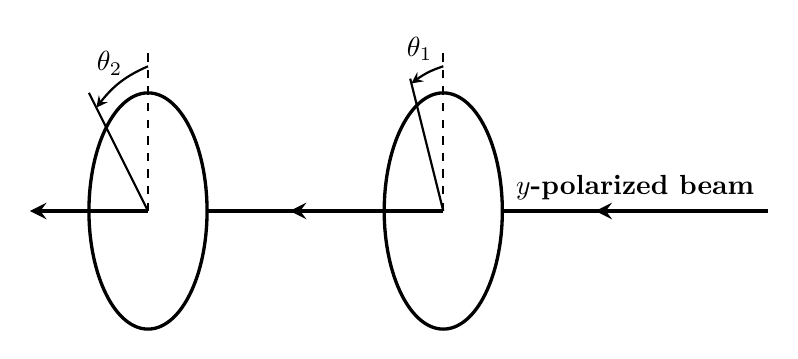
\begin{tikzpicture}[scale=0.75, decoration={markings,
        mark= at position 0.65 with {\arrow{stealth}}}]
                \draw[very thick] (0,0) ellipse (1cm and 2cm);
                \draw[very thick] (5,0) ellipse (1cm and 2cm);
                \draw[ultra thick, postaction={decorate}] (10.5,0) -- (6,0) node[midway, above] {$y$\textbf{-polarized beam}};
                \draw[ultra thick, postaction={decorate}] (5,0) -- (1,0);
                \draw[ultra thick, -stealth] (0,0) -- (-2,0);
                \draw[thick, dashed] (0,0) -- (0,2.75) (5,0) -- (5,2.75);
                \draw[thick] (0,0) -- (-1,2) (5,0) -- (4.44, 2.24);
                \draw[thick, -stealth] (0,2.45) to[bend right=15] (-0.875, 1.75);
                \node at (-0.65,2.5) (tt) {$\theta_2$};
                \draw[thick, -stealth] (5,2.45) to[bend right=10] (4.46,2.16);
                \node at (4.6,2.75) (t) {$\theta_1$};
        \end{tikzpicture}
    \end{center}

    \begin{enumerate}
        \item What is the transmission probability through the \textit{first} polarizer, for $\theta_1 = 0$? for $\theta_1 = \pi/2$?
        
        \begin{solution}
            Here, all the light passes thorugh for $\theta_1 = 0$, since the linear polarizer is aligned perfectly with the light. In the case where $\theta_1 = \pi/2$, we get no light passing through, since all the light is initially y-polarized.
        \end{solution}
        \item What is the net transmission probability through the system of \textit{two polarizers}: 
        \begin{itemize}
            \item for $\theta_1 = 0$ and $\theta_2 \neq 0$?
            \item for $\theta_1 = \theta_2$?
            \item for $\theta_1 = \theta_2/2$?
            
            \begin{solution}
                For $\theta_1 = 0$ and $\theta_2 \neq 0$, we get that the probability is $\cos^2(\theta_2)$, since all the light passes through the first lens so the only part that actually gets filtered is through the second lens.

                For $\theta_1 = \theta_2$, the probability is going to be $\cos^2(\theta_1)$, since any light that passes through the first polarizer is now guaranteed to pass through the second polarizer.

                For $\theta_1 = \theta_2/2$, we have the transmission probability is the product of the two transmission probabilities, in other words: 
                
                \[ T = \cos^2(\theta_1) \cdot \cos^2(\theta_2 - \theta_1)\]

                And since $\theta_2 = 2\theta_1$, then this equation simplifies to 

                \[ T = \cos^4(\theta_1)\]
            \end{solution}
        \end{itemize}
        \item Find an expression for the net transmission probability through the system as a function of $\theta_1$ for a given fixed value of $\theta_2$. For what value(s) of $\theta_1$ is the transmission a maximum?
        
        \begin{solution}
            We have the transmission probability is: 

            \[ T = \cos^2 \theta_1 \cdot \cos^2(\theta_2 - \theta_1)\] 

            And so we can take the derivative: 

            \begin{align*}
                \frac{\partial T}{\partial \theta_1} = 0 &= 2\cos(\theta_1) (-\sin \theta_1)\cos^2(\theta_2 - \theta_1) + \cos^2 \theta_1 \cdot 2\cos(\theta_2 - \theta_1) \cdot \sin (\theta_2 - \theta_1)\\
                \sin \theta_1 \cos(\theta_2 - \theta_1) &= \cos(\theta_1)\sin(\theta_2 - \theta_1)\\
                \tan(\theta_1) &= \tan(\theta_2 -\theta_1)\\
                \therefore \theta_1 &= \frac{\theta_2}{2}
            \end{align*}

            which gives us the optimal transmisison angle to be $\theta_1 = \frac{\theta_2}{2}$z
        \end{solution}
    \end{enumerate}

    \pagebreak 

    \section*{Problem 5}
    In a low-intensity counting experiment a weak beam of right-circularly polarized light enters an $xy$ analyzer. In a given experimental run 54 photons are counted in the $x$ output channel and 46 in the $y$-output channel. The experimenter concludes that the incident beam cannot be $R$ polarized since, he says, an $R$-polarized beam should yield equal intensities in the $x$ and $y$ channels.

    \begin{enumerate}[(a)]
        \item Make a brief, but if possible, quantitative argument that the experimental result is not consistent with the incident beam being in the $R$-polarized state. 
        
        \begin{solution}
            The crucal bit here is tha the beam is weak, meaning we can think of this experiment as transmitting individual photons. Therefore, we can think of the photons as discrete particles with a certain period in its oscillation.
            
            The beam can still be $R$-polarized, because we could be measuring the light at a point wehre the polarization is in a superposition of $x$ and $y$.
        \end{solution}
        \item What alternative experiment would you propose in which detection of 100 photons would provide more convincing evidence that the incident beam is $R$ polarized? What would you expect for your proposed experiment? Would such an outcome make it \textit{certain} that the incident beam is $R$ polarized?
        
        \begin{solution}
            We could perform the same experiment but measure the light beam at distances where they are not multiples of any previous distance we measure (in other words, they must all be relatively prime). That way, if the light is truly circularly polarized, we would obtain a different distribution for every measurement. 

            That said, we can never be certain about the nature of the light, because for any finite number of lengths, we could find a wavelength of light such that the experiment outputs the same distribution for all measurements. In order to be certain, we require an infinite number of measurements to be made.
        \end{solution}
    \end{enumerate}
\end{document}